\documentclass{xtupaper}
\usepackage[urlcolor=blue]{hyperref}
\usepackage{threeparttable}
\usepackage{setspace}
\usepackage{titlesec}
\usepackage{float}
\newcommand{\upcite}[1]{\textsuperscript{\textsuperscript{\cite{#1}}}}
\usepackage{fancyhdr}
\titleformat{\section}{\large \heiti}{\chinese{section}、}{0em}{}
\begin{document}
\begin{center}
\LARGE
  \textbf{数值积分——复化Simpson求积公式}\\
  \vspace{0.5em}
  \large
湘潭大学,\ 数学与计算科学学院,21级王艺博
  \end{center}
\rule[0.1\baselineskip]{\textwidth}{0.5pt}

\section{复化Simpson求积公式}

Simpson公式
\[\int_a^bf(x)\mathrm{d}x\approx\frac{b-a}{6}\left(f(a)+4f\left(\frac{a+b}{2}\right)+f(b)\right).\]
 
把积分区间$[a,b]$进行$2m$(偶)等分,记$n = 2m$,其中 $n+1$是节点总数,$m$是积分子区间的总数.

步长$h=\frac{b-a}{n}$,节点$x_{k}=a+kh,(k=0,1,2,\cdots,n)$

\[\int_{a}^{b}f(x)\mathrm{d}x=\sum_{i=0}^{m-1}\int_{x_{2i}}^{x_{2i+2}}f(x)\mathrm{d}x\]

	
	在$ [x_{2i},x_{2i+2}] $上用Simpson公式
	\[\int_{x_{2i}}^{x_{2i+2}}f(x)\mathrm{d}x \approx \frac{h}{3}[f(x_{2i})+4f(x_{2i+1})+f(x_{2i+2})] \]

\textbf{累加得复化Simpson求积公式}
	\[S_n(f) \approx\frac{h}{3}\left[f(a)+4\sum_{i=0}^{m-1}f(x_{2i+1})+2\sum_{i=1}^{m-1}f(x_{2i})+f(b)\right]\]
\newpage
\section{算法}

$\heartsuit$ 复化Simpson积分:\verb|  S = 复化Simpson_v1(a,b,n,f)|
\begin{enumerate}
	\item 输入
		
		\begin{itemize}
					\item  $[a,b]$
					
					\item  n : 将[a,b] $n$等分 ,要求$ n $为偶数
					
					\item f : 已经定义好的函数,支持向量运算
					
		\end{itemize}


	\item 实现过程
			\begin{itemize}
						\item  判断$n$是否是偶数,若不是,$+1$变为偶数
						
						\item  m = n/2;
						
						\item 计算出 $[a, b] n$ 等分后得到的 $n + 1$ 个节点,构成向量 x0
						\item y0 = f(x0)
						
			\end{itemize}
	
	  \[sumy1 = \sum_{i=0}^{m-1}f(x_{2i+1}) \]
	\[ sumy2 = \sum_{i=1}^{m-1}f(x_{2i}) \] 
	\[S =\frac{h}{3}\left[f(a)+4*sumy1+2*sumy2+f(b)\right]\]

	\item 输出 S

\end{enumerate}

%\begin{algorithm}[h]
%	\caption{ 分段线性插值\_v1 思路}
%	\begin{algorithmic}[1]
%		\Require  x0(样本点横坐标向量),y0(样本点纵坐标向量),x(所求点)
%		\Ensure   y(x对应的近似值)
%		\State n1,n2 表示 x0,x 向量的长度,设基函数向量为 $ l $ 
%		\For {k=1:1:n2}   \Comment{对每一个x计算对应的基函数}
%			\If{$ x_0\leqslant x\leqslant x_1 $}\Comment{首端}
%				\State $ l(1) = \frac{x-x_1}{x_0-x_1} $
%			\ElsIf{$ x_1<x\leqslant x_n $}
%				\State$ l(1) = 0 $
%			\EndIf
%			
%			\For {i=1:1:n-1}\Comment{中间}
%				\If{$ x_{i-1} \leqslant x \leqslant x_i $}
%					\State	$ l(i) = \frac{x - x_{i-1}}{x_j - x_{i-1}} $
%				\ElsIf{$ x_i < x \leqslant x_{i+1} $}
%					\State	$ l(i) = \frac{x - x_{i+1}}{x_j - x_{i+1}} $
%				\ElsIf{others}
%					\State	$ l(i) = 0$
%				\EndIf
%			\EndFor
%			
%			\If{$ x_{n-1}\leqslant x\leqslant x_{n} $}\Comment{末端}
%				\State $ l(n) = \frac{x-x_{n-1}}{x_{n}-x_{n-1}}$
%			\ElsIf {$ x_0 < x \leqslant x_{n-1} $}
%				\State  $ l(n) = 0$
%			\EndIf			
%			\State $ y(j) = y0*l' $ 
%		\EndFor
%	\end{algorithmic}
%\end{algorithm}

\newpage
\section{北太天元源程序}
\begin{lstlisting}[language=matlab]
function S = 复化Simpson_v1(a,b,n,f)
% [a,b]
% n :小区间的个数, 要求是偶数
% f:定义好的函数
    if mod(n,2) != 0    % 判断n是否为偶数,如果不是,使其变为偶数
    	   n = n+1;
    end
    h = (b-a)/n;
    k = 0:1:n;    
    xi = a + k * h;
    yi = f(xi);
    m = n/2;
    i1 = 0:1:m-1;
        sumy1 = sum(yi(2*i1+1 +1)); % f(x_{2i+1})求和
    i2 = 1:1:m-1;       
        sumy2 = sum(yi(2*i2 +1)); % f(x_{2i})求和
    S = (yi(1) + 4*sumy1 + 2*sumy2 + yi(n+1)) * h/3;
end
\end{lstlisting}
将上述代码保存为\verb| 复化Simpson_v1.m |文件。

\newpage
\section{数值算例}
\begin{example}\label{exmT1} 
用数值积分法近似计算
\[\pi = 4\int_0^1 \frac{1}{1+x^2}\mathrm{d}x\]
编写复化Simpson公式的实现程序,分别取剖分段数 $ n = 10, 20, 40, 80, 160, $ 计算积分值与 $\pi$ 的误差并作图;
\end{example}

\paragraph{例子}

\begin{lstlisting}[language=matlab]
% 复化Simpson求积例子
clc;clear all;format long;
f = @(x) 4./(1+x.^2);

N = [10 20 40 80 160];
delta = zeros(1,5);
k = 1;
for n = N
    S = 复化Simpson_v1(0,1,n,f);
    delta(k) = abs(pi - S);
    k++;
end
    	plot(N,delta,'b');
disp(delta);
    
    
\end{lstlisting}
将上述代码保存为 \verb| 复化Simpson例子.m |

\paragraph{运行后得到}
积分值与 $ \pi $的误差
\begin{verbatim}
  列 1 -- 3
   0.000000039650578   0.000000000620008   0.000000000009688   
  列 3 -- 5
   0.000000000000151   0.000000000000002
\end{verbatim}

\begin{figure}[htp]%H表示图强制在下面,想设置浮动环境用htp
	\centering  %插入的图片居中表示
	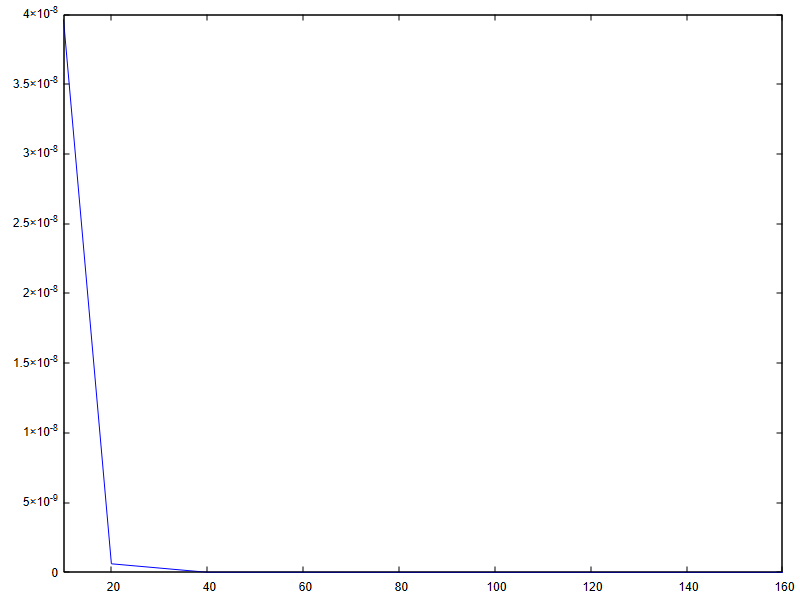
\includegraphics[scale=0.5]{Sm1} 
	\caption{复化Simpson求积公式下 积分值与 $ \pi $的误差随n的变化}  %图片的名称
	\label{Sm1}
\end{figure}
\begin{figure}[htp]%H表示图强制在下面,想设置浮动环境用htp
	\centering  %插入的图片居中表示
	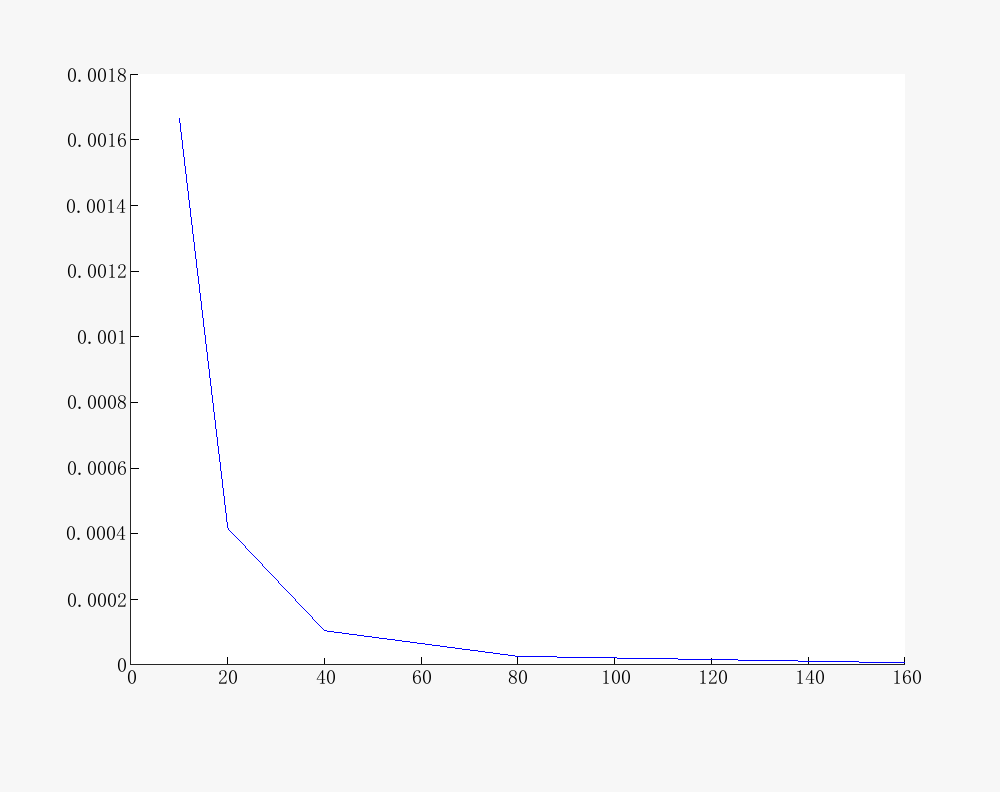
\includegraphics[scale=0.5]{tixing1} 
	\caption{复化梯形求积公式下 积分值与 $ \pi $的误差随n的变化}  %图片的名称
	\label{tx1}
	

\end{figure}
		从图像可知,复化Simpson收敛速度更快
\begin{figure}[htp]%H表示图强制在下面,想设置浮动环境用htp
	\centering  %插入的图片居中表示
	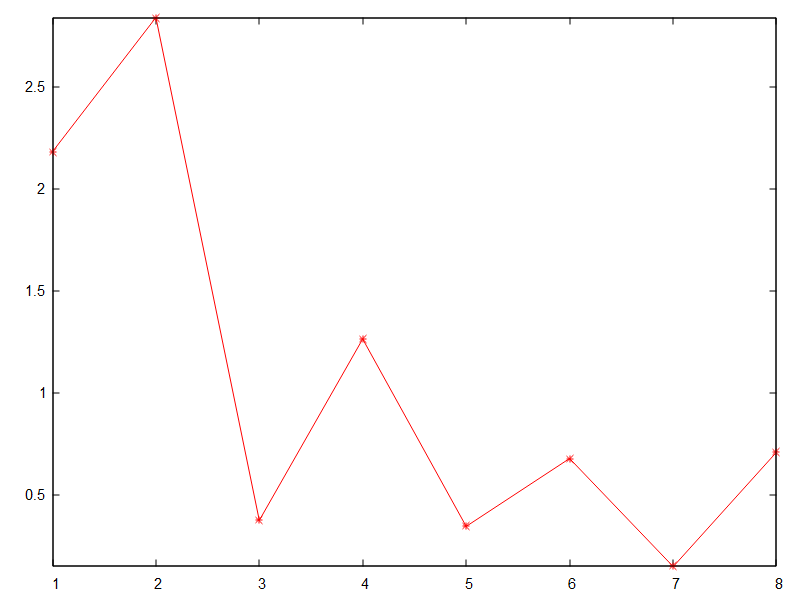
\includegraphics[scale=0.5]{NC2} 
	\caption{Newton—Cotes公式下的一个图像参照}  %图片的名称
	\label{NC2}
	

\end{figure}


\end{document} 
